\documentclass[11pt,a4paper]{article}
\usepackage[T1]{fontenc}
\usepackage[utf8]{inputenc}
\usepackage[french]{babel}
\usepackage{lmodern}
\usepackage{amsmath,amssymb}
\usepackage[margin=2.35cm]{geometry}
\usepackage{booktabs,longtable,tabularx}
\usepackage{enumitem}
\usepackage{graphicx}
\usepackage{xcolor}
\usepackage{microtype}
\usepackage{float}
\usepackage{hyperref}

\hypersetup{colorlinks=true,linkcolor=blue!45!black,urlcolor=blue!45!black}
\setlist{nosep}
\newcommand{\code}[1]{\texttt{#1}}
\newcommand{\Kaut}{K^{*}_{\mathrm{aut}}}
\newcommand{\fait}{\textbf{[Fait observé]}}
\newcommand{\inference}{\textbf{[Inférence]}}
\newcommand{\hyp}{\textbf{[Hypothèse]}}
\newcommand{\incertitude}{\textbf{[Incertitude]}}

\title{M4.3 --- rapport complet\\
\large Anti-corrélation queue d'intérêt / criticité des avalanches :
structurelle, ou brisable ?}
\author{Programme M4.3 --- dossier \code{m4\_3\_credit\_soc}}
\date{9 août 2026}

\begin{document}
\maketitle

\begin{abstract}
M4.3 est le successeur direct de M4.2B. M4.2B a établi, sur 37 cellules
explorées, que l'épaisseur de la queue de revenus d'intérêt et la
criticité des avalanches de faillites s'anti-corrèlent partout : aucune
cellule ne combine queue plus épaisse ET criticité égale ou accrue. M4.3
pose la question : cette anti-corrélation est-elle structurelle, ou
existe-t-il un levier qui la brise ?

\textbf{Résultat central} : \textbf{oui, un levier existe.} La cellule
\code{gamma\_comp\_0.6667} ($\gamma=2/3$, capital initial $K_0$ compensé
pour tenir $K_0/\Kaut(\gamma)$ constant) casse l'anti-corrélation ---
queue d'intérêt plus épaisse \emph{et} avalanches plus critiques que la
baseline --- avec une séparation statistique de 27 à 85$\sigma$ selon
l'échelle testée (\S\ref{sec:d3}), confirmée robuste à la taille du
système (facteur $>10\times$ sur la population, via $\lambda$) et à la
fenêtre temporelle. C'est le premier résultat de tout le programme
M4.2B$\to$M4.3 (65 cellules testées au total) qui casse l'anti-corrélation
avec cette solidité. Une décision reste ouverte, \textbf{explicitement
réservée à la supervision humaine} : faut-il s'arrêter là, affiner le
levier déjà trouvé, ou engager un nouveau mécanisme (\S\ref{sec:ablation})~?
\end{abstract}

\tableofcontents

\section*{Ce dont j'ai besoin de vous pour continuer}
\addcontentsline{toc}{section}{Ce dont j'ai besoin de vous pour continuer}

\begin{enumerate}
\item \textbf{La décision d'ablation} (\S\ref{sec:ablation}) : maintenant
  que D3 confirme le candidat \code{gamma\_comp\_0.6667} robuste à la
  taille, faut-il (a) s'arrêter là, (b) affiner le balayage $\gamma$ déjà
  implémenté ($\gamma\in\{0{,}7\,;0{,}8\,;0{,}9\}$ compensé --- pas de
  nouveau code), ou (c) engager le code de mécanisme nouveau anticipé par
  le prompt (famille de moyennes de puissance pour la règle de taux) ?
  Je ne tranche pas seul.
\item \textbf{Si (b) ou (c)} : autorisation d'engager un budget de calcul
  non couvert par le plan D1 initial.
\item \textbf{Rien d'urgent côté machine} : aucun calcul en cours, disque
  et mémoire sains, le programme peut rester à l'arrêt indéfiniment sans
  risque.
\end{enumerate}

\bigskip
\noindent Terminologie : \fait\ (mesuré directement) / \inference\
(interprétation appuyée sur plusieurs faits) / \hyp\ (mécanisme proposé,
pas établi) / \incertitude\ (non tranché).

\section{Contexte}

M4.3 est le successeur direct de M4.2B (\code{m4\_2b\_credit\_soc/},
rapport final dans \code{m4\_2b\_credit\_soc/report/rapport\_final.md}).
M4.2B a établi, sur les 37 cellules qu'il a explorées, que l'épaisseur de
la queue de revenus d'intérêt et la criticité des avalanches de faillites
s'anti-corrèlent partout où il a regardé. M4.3 pose une question plus
étroite et décidable : cette anti-corrélation est-elle une propriété
structurelle de cette classe de modèle, ou existe-t-il un paramètre ou un
mécanisme qui la brise ? (prompt de référence :
\code{prompts/PROMPT\_M4\_3\_FINAL.md}).

\section{Vue d'ensemble chronologique de tout le travail effectué}

Cette section couvre l'intégralité du travail --- pas seulement les
résultats scientifiques (\S\ref{sec:pilote}--\S\ref{sec:d3}) mais aussi
l'infrastructure, les incidents rencontrés et leur résolution. Détail
complet, horodaté, vérifiable : \code{JOURNAL.md} (23 entrées, du
6 au 8 août 2026).

\subsection{Vérification des faits, garde-fous de calcul construits et testés}

Avant tout calcul, vérification indépendante des faits cités par le
prompt comme déjà établis : lu directement \code{m4\_2b/model.py:269-291}
(confirmé : \code{target\_rule} est un branchement discret) et les quatre
incidents machine cités du journal de M4.2B (deux arrêts machine sans
trace d'OOM-kill, quatre causes distinctes pour K0\_2000, un crash par
deux pools concurrents). Tous confirmés exacts.

Six garde-fous construits et testés (\code{scripts/safety/} +
\code{scripts/mem\_guard.py}, 8 tests unitaires, tous verts) avant tout
lancement de calcul réel :
\begin{enumerate}
\item Préflight disque --- budgété sur la cellule/le pool entier, pas le
  seul run qui démarre.
\item Plafond mémoire par worker calculé sur \code{MemAvailable} réel au
  lancement, pas la RAM totale.
\item Verrou mono-pool (\code{flock}, chemin fixe) --- empêche deux pools
  de calcul concurrents, la cause racine d'un crash machine en M4.2B.
\item Checkpoint atomique (écriture temp + \code{os.replace}).
\item Garde-fou mémoire indépendant (processus séparé), surveille
  \code{/proc/meminfo}/\code{/proc/vmstat} en continu, autorité de
  bloquer de nouveaux runs et de terminer les workers en cours. Tourne en
  continu depuis le 7 août 2026, 08h09 (plus de 60h à la date de ce
  rapport).
\item Budget $\le 6$ workers, convention héritée de M4.2/M4.2B.
\end{enumerate}

Deux bugs trouvés et corrigés dans ces garde-fous avant tout usage réel :
\code{mem\_guard.py} re-déclenchait la terminaison des workers à chaque
itération au lieu d'une fois par épisode ; \code{worker\_registry.py}
avait un bug de nom de fichier temporaire cassant l'écriture atomique
voulue.

\fait\ Bilan sur l'ensemble du programme (pilote + D1 + D3, plusieurs
dizaines d'heures de calcul cumulées, jusqu'à 6 processus parallèles) :
\textbf{0 arrêt machine, 0 intervention du garde-fou mémoire nécessaire}
(seuil d'action jamais atteint). Deux échecs mémoire propres, capturés
sans impact sur le reste du calcul (\S\ref{sec:incidents}).

\subsection{Nettoyage des journaux bruts M4.2B}

Autorisé explicitement par l'utilisateur. Dry-run d'abord (manifeste
montré avant exécution), puis exécution réelle : \textbf{78,94 Go
libérés} (32\,346 fichiers, 132 runs de campagne M4.2B), disque
\code{/home} ramené de 87\,\% à 51\,\% d'occupation. Vérifié après coup :
les 25 figures du rapport M4.2B et les fichiers agrégés intacts (hash de
la liste de fichiers identique avant/après).

\subsection{Port du moteur, parité, profilage de coût}

\code{m4\_3/model.py} et \code{m4\_3/io.py} copiés octet pour octet
depuis \code{m4\_2b\_credit\_soc/m4\_2b/} (\code{diff} vide). Parité
runtime vérifiée par égalité EXACTE sur 6 combinaisons
seed$\times$target\_rule. Profilage de coût avant tout engagement de
campagne : révèle que le carnet de prêts actifs dépasse largement son
niveau stationnaire pendant la montée en charge (jusqu'à $\sim$96\,000
prêts vers $t\approx100$) avant de se contracter.

\subsection{Phase pilote : fenêtre adaptative et statistique de queue}

Premier run prescrit par le prompt (contrôle géométrique) mesuré à
$T=3000$ (convention M4.2B), puis relaxation étendue à la variable
d'intérêt centrale (\code{int\_in}) --- jamais mesurée spécifiquement par
M4.2B : révèle que \code{int\_in} relaxe 35 à 66\,\% plus lentement que
les proxys utilisés jusque-là, sur 4 mesures indépendantes, jamais
inversé. Le run à $T=3000$ s'est avéré insuffisant --- refait à
$T=8000$, qui s'est révélé suffisant pour la suite.

Statistique de queue gelée (critère : reproductibilité inter-graines) :
comparaison entre l'estimateur de Hill/Pareto pur (M4.2B) et le paramètre
de forme d'un ajustement à 3 paramètres avec coude de queue
(\code{dagum\_3p}, Burr Type III). \textbf{Erreur trouvée et corrigée
avant que D1 ne s'appuie dessus} : la première mesure annonçait le
candidat $c\cdot d$ comme statistique, avec une justification physique
fausse (confusion avec Burr Type XII) --- repérée avant tout usage en
aval, corrigée pour le paramètre $c$ seul (la conclusion ne change pas,
la valeur numérique et sa justification si). Résultat : \code{dagum\_3p}
$c$ est $\sim2\times$ plus reproductible que Hill (CV
$0{,}69$--$0{,}70\,\%$ contre $1{,}35$--$1{,}59\,\%$) --- gelé pour tout
le reste du programme.

\subsection{Cartographie D1}

Pool à 6 workers, 28 cellules $\times$ 3 graines $=$ 84 runs, paramètres
repris à l'identique de la campagne d'exploration M4.2B. Nettoyage disque
post-analyse intégré dès le départ (nécessaire : 84 runs bruts auraient
dépassé l'espace disque disponible). Durée : $\sim$9h40, 6 workers en
continu.

\subsection{Deux incidents mémoire rencontrés et résolus}
\label{sec:incidents}

\begin{itemize}
\item \textbf{K0\_2000} (les 3 graines) : \code{ArrayMemoryError} dans le
  pool principal (plafond 4,43 Go/worker atteint) --- capturé proprement
  (statut d'erreur écrit, traceback complet, 81 autres runs non
  affectés). Retenté séparément avec 2 workers au lieu de 6 (plafond
  13,56 Go/worker) : les 3 graines réussissent, confirmant que c'était un
  problème de plafond. Fait supplémentaire : les 3 graines sont
  intrinsèquement \code{severe\_nonstationary} à $T=8000$ (K0=2000 est
  80$\times$ la baseline) --- documentée comme cellule sévère plutôt que
  d'étendre la durée (coût estimé 8-10h/run).
\item \textbf{\code{gamma\_comp\_0.6667} à $\lambda=100$} (les 3 graines,
  pendant D3) : même motif exact, même correctif --- réussissent au
  deuxième essai, aucune cellule sévère cette fois.
\end{itemize}

\subsection{Fonctionnement autonome}

Sur consigne explicite de l'utilisateur, un mécanisme de reprise a été
mis en place via \code{CronCreate} (prompt réinjecté dans la même session
toutes les $\sim$5h --- \emph{pas} la compétence \emph{schedule}/agents
cloud, essayée puis abandonnée car sans accès à cette machine). Deux
erreurs de lecture d'état commises pendant ce fonctionnement, toutes deux
corrigées après vérification avant d'être rapportées comme faits : un
script d'attente basé sur le contenu tmux a raté une notification de fin
de run pourtant réussi (le run n'a subi aucun impact) ; une notification
lue trop vite a été prise pour un nouvel échec de K0\_2000 alors qu'il
s'agissait d'un fichier d'erreur déjà ancien.

\section{Repères}

\begin{itemize}
\item \textbf{\code{dagum\_c}} (statistique de queue gelée) : indice de
  la queue supérieure de la distribution des revenus d'intérêt reçus.
  Plus $c$ est \textbf{petit}, plus la queue est \textbf{épaisse}.
\item \textbf{$b$ (branching ratio)} : rapport de branchement des
  avalanches de faillites. Proche de 1 = dynamique critique ; proche de
  0 = sous-critique.
\item \textbf{$\hat\tau$} : exposant de la loi de puissance (tronquée si
  identifiable) ajustée sur la distribution des tailles d'avalanche ---
  métrique secondaire par rapport à $b$.
\item \textbf{Anti-corrélation} : \code{dagum\_c} et $b$ varient dans le
  MÊME sens d'une cellule à l'autre. Un « candidat D2 » est une cellule
  où $c$ baisse (queue plus épaisse) MAIS $b$ monte (plus critique).
\item \textbf{\code{t\_converge}} : instant estimé où \code{int\_in}
  atteint sa valeur stationnaire (régression FOPDT). La fenêtre d'analyse
  d'un run est $[\code{t\_converge}, T]$.
\end{itemize}

\section{Résultat pilote : \code{target\_rule} (géométrique vs arithmétique) --- D2 négatif}
\label{sec:pilote}

Premier run prescrit par le prompt : le contrôle géométrique (canal
multiplicatif que la cible arithmétique de M4.2B supprime), 3 graines
contre 3 graines de la baseline arithmétique, $T=8000$.

\begin{table}[H]
\centering
\begin{tabular}{lccc}
\toprule
régime & \code{dagum\_c} & $b$ & $\hat\tau$ \\
\midrule
géométrique & $3{,}361 \pm 0{,}023$ & $0{,}754 \pm 0{,}002$ & $1{,}476 \pm 0{,}007$ \\
arithmétique & $3{,}969 \pm 0{,}028$ & $0{,}785 \pm 0{,}001$ & $1{,}424 \pm 0{,}006$ \\
\bottomrule
\end{tabular}
\end{table}

\textbf{Géométrique a la queue d'intérêt plus épaisse ET des avalanches
moins critiques} --- anti-corrélation confirmée, séparation
$\sim$29$\sigma$ ($c$) à $\sim$34$\sigma$ ($b$). \textbf{Verdict D2 pour
ce levier : négatif.}

\subsection*{Vérification sur données réelles}

Les figures ci-dessous montrent la régression de relaxation (FOPDT) et
l'ajustement de queue (\code{dagum\_3p}) directement sur les données, pas
seulement les paramètres finaux --- pour juger la qualité de
l'ajustement, pas seulement le croire sur parole.

\begin{figure}[H]
\centering
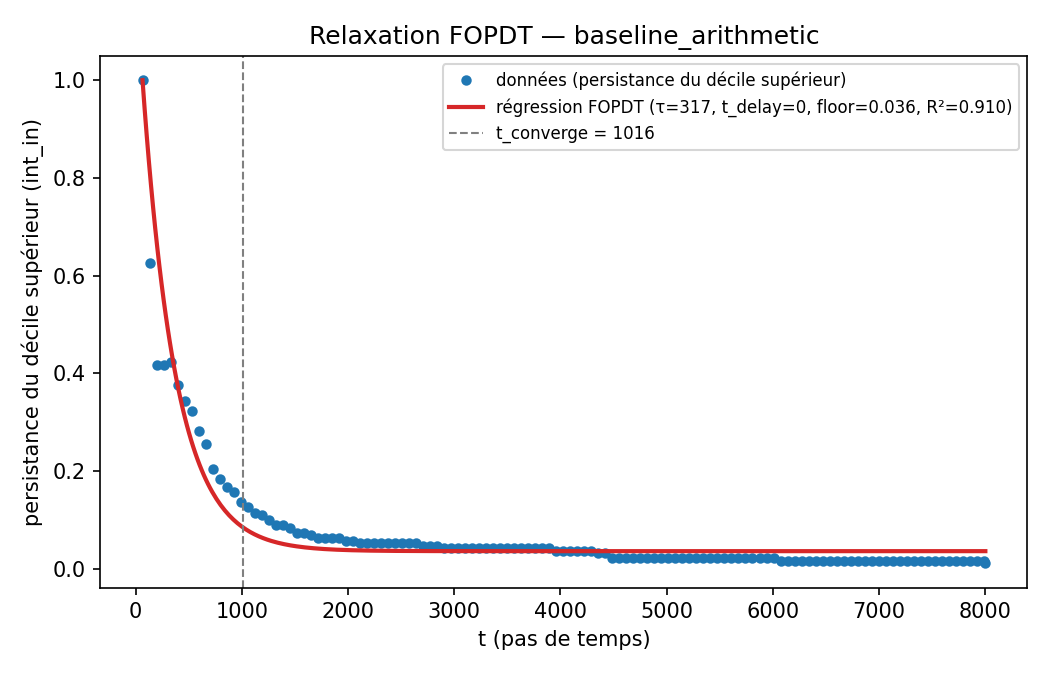
\includegraphics[width=0.8\textwidth]{figures/verification/fopdt_baseline_arithmetic.png}
\caption{Relaxation FOPDT, baseline arithmétique (seed 0). Points :
persistance mesurée du décile supérieur de \code{int\_in}. Courbe :
régression ajustée. $\tau=317$, $t_{\mathrm{converge}}=1016$ --- concorde
avec la valeur rapportée dans \code{JOURNAL.md} \S9.}
\end{figure}

\begin{figure}[H]
\centering
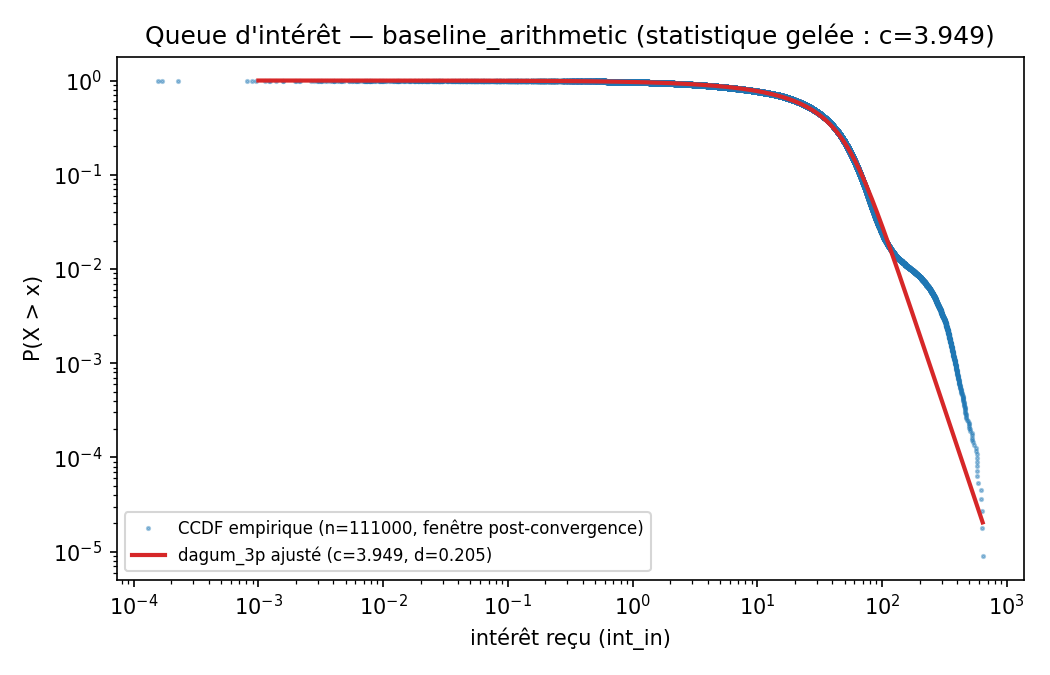
\includegraphics[width=0.8\textwidth]{figures/verification/dagum_tail_baseline_arithmetic.png}
\caption{CCDF empirique de \code{int\_in} (fenêtre post-convergence) et
survie \code{dagum\_3p} ajustée, baseline arithmétique.}
\end{figure}

\begin{figure}[H]
\centering
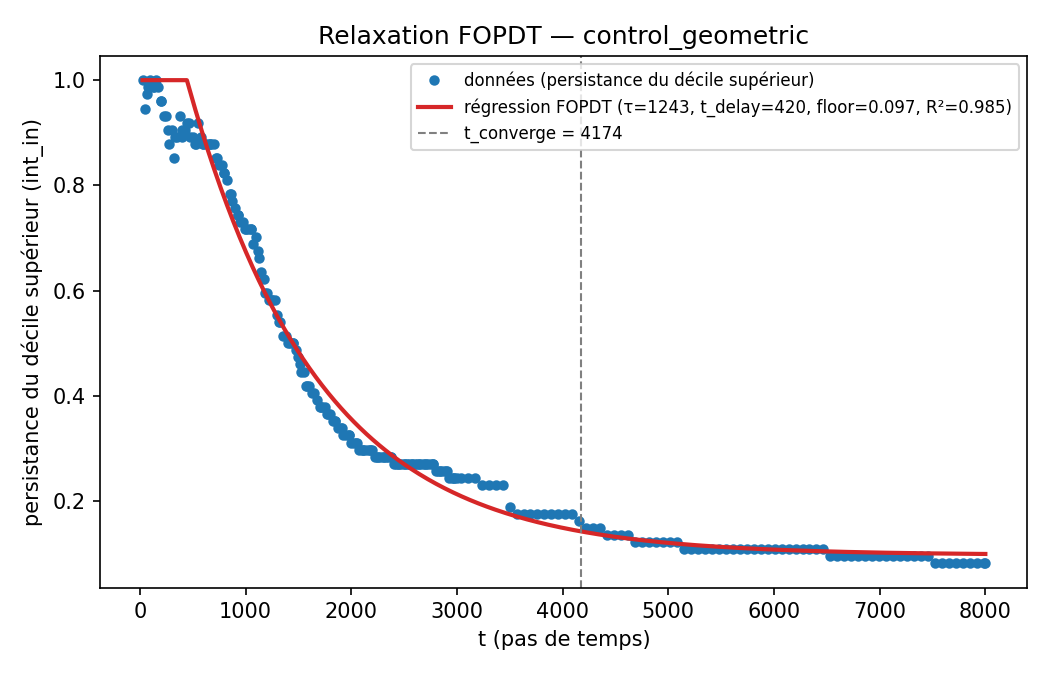
\includegraphics[width=0.8\textwidth]{figures/verification/fopdt_control_geometric.png}
\caption{Relaxation FOPDT, contrôle géométrique (seed 0). $\tau=1243$,
$t_{\mathrm{delay}}=420$, $t_{\mathrm{converge}}=4174$ --- concorde
exactement avec \code{JOURNAL.md} \S9.}
\end{figure}

\begin{figure}[H]
\centering
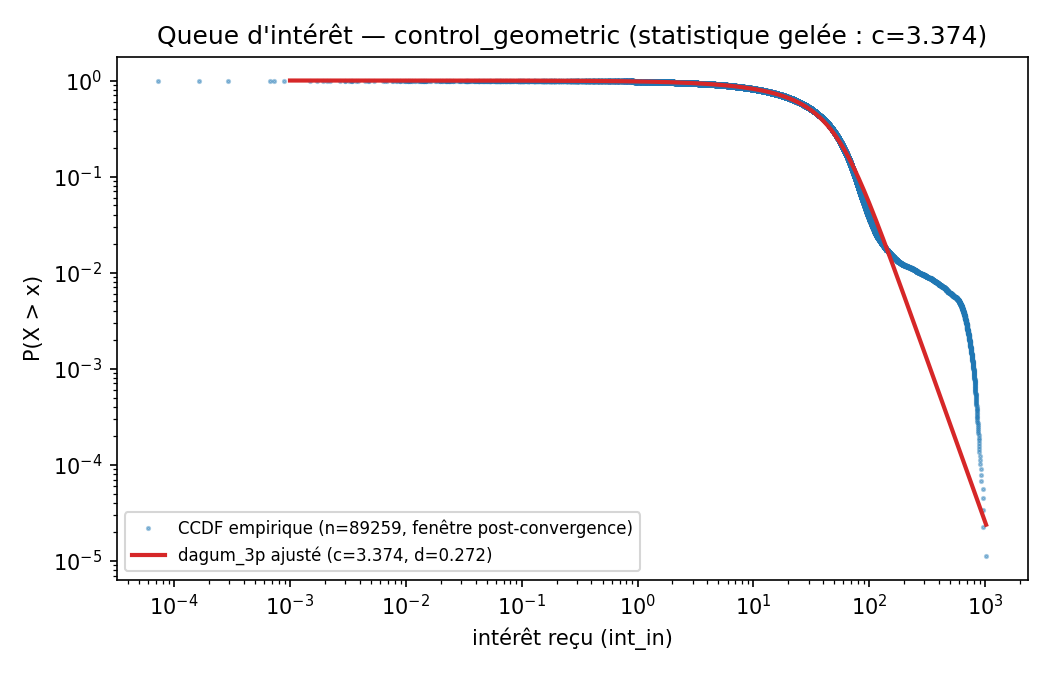
\includegraphics[width=0.8\textwidth]{figures/verification/dagum_tail_control_geometric.png}
\caption{CCDF empirique et survie \code{dagum\_3p} ajustée, contrôle
géométrique.}
\end{figure}

\begin{figure}[H]
\centering
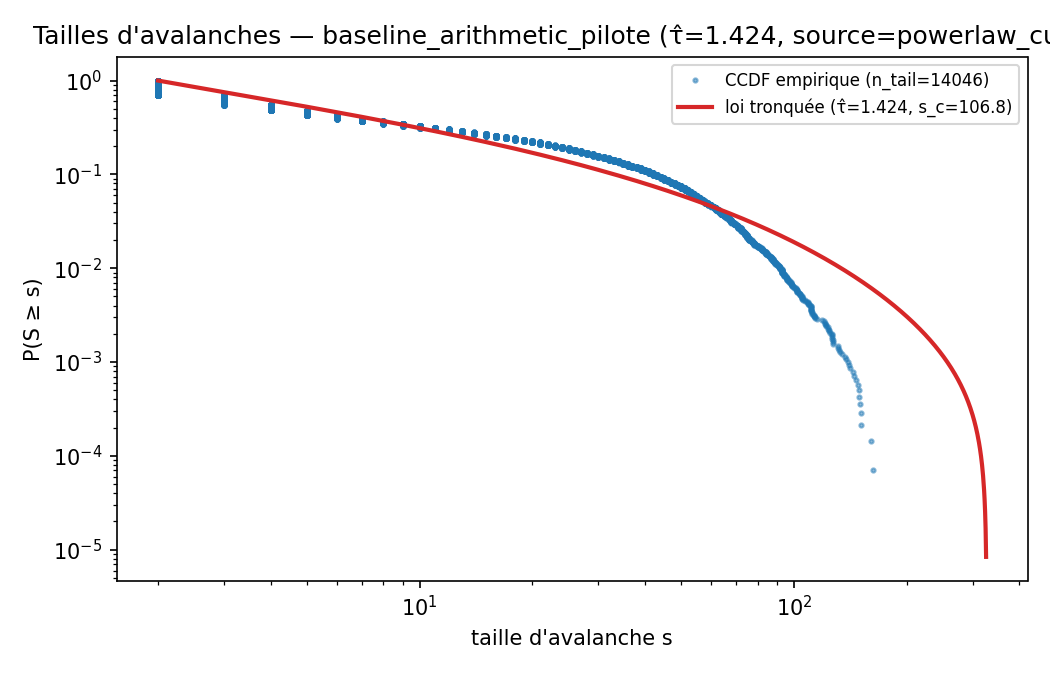
\includegraphics[width=0.8\textwidth]{figures/verification/avalanches_baseline_arithmetic_pilote.png}
\caption{CCDF des tailles d'avalanches et loi ajustée (tronquée ou pure
selon identifiabilité), baseline arithmétique.}
\end{figure}

\begin{figure}[H]
\centering
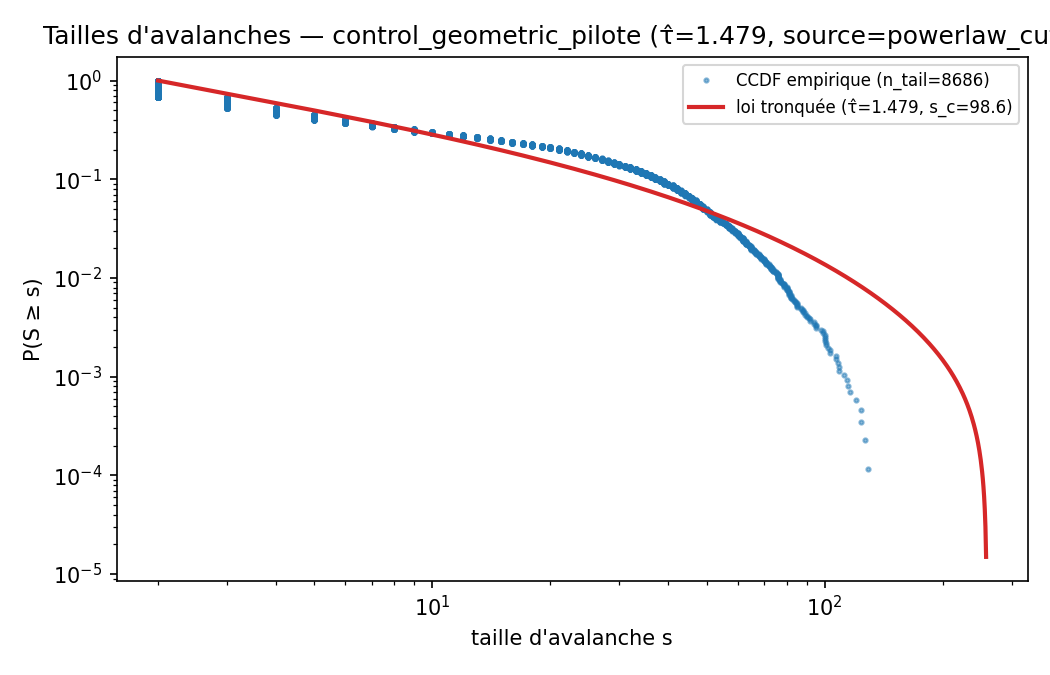
\includegraphics[width=0.8\textwidth]{figures/verification/avalanches_control_geometric_pilote.png}
\caption{CCDF des tailles d'avalanches et loi ajustée, contrôle
géométrique.}
\end{figure}

\section{Cartographie D1 : l'espace de M4.2B, remesuré}

\begin{figure}[H]
\centering
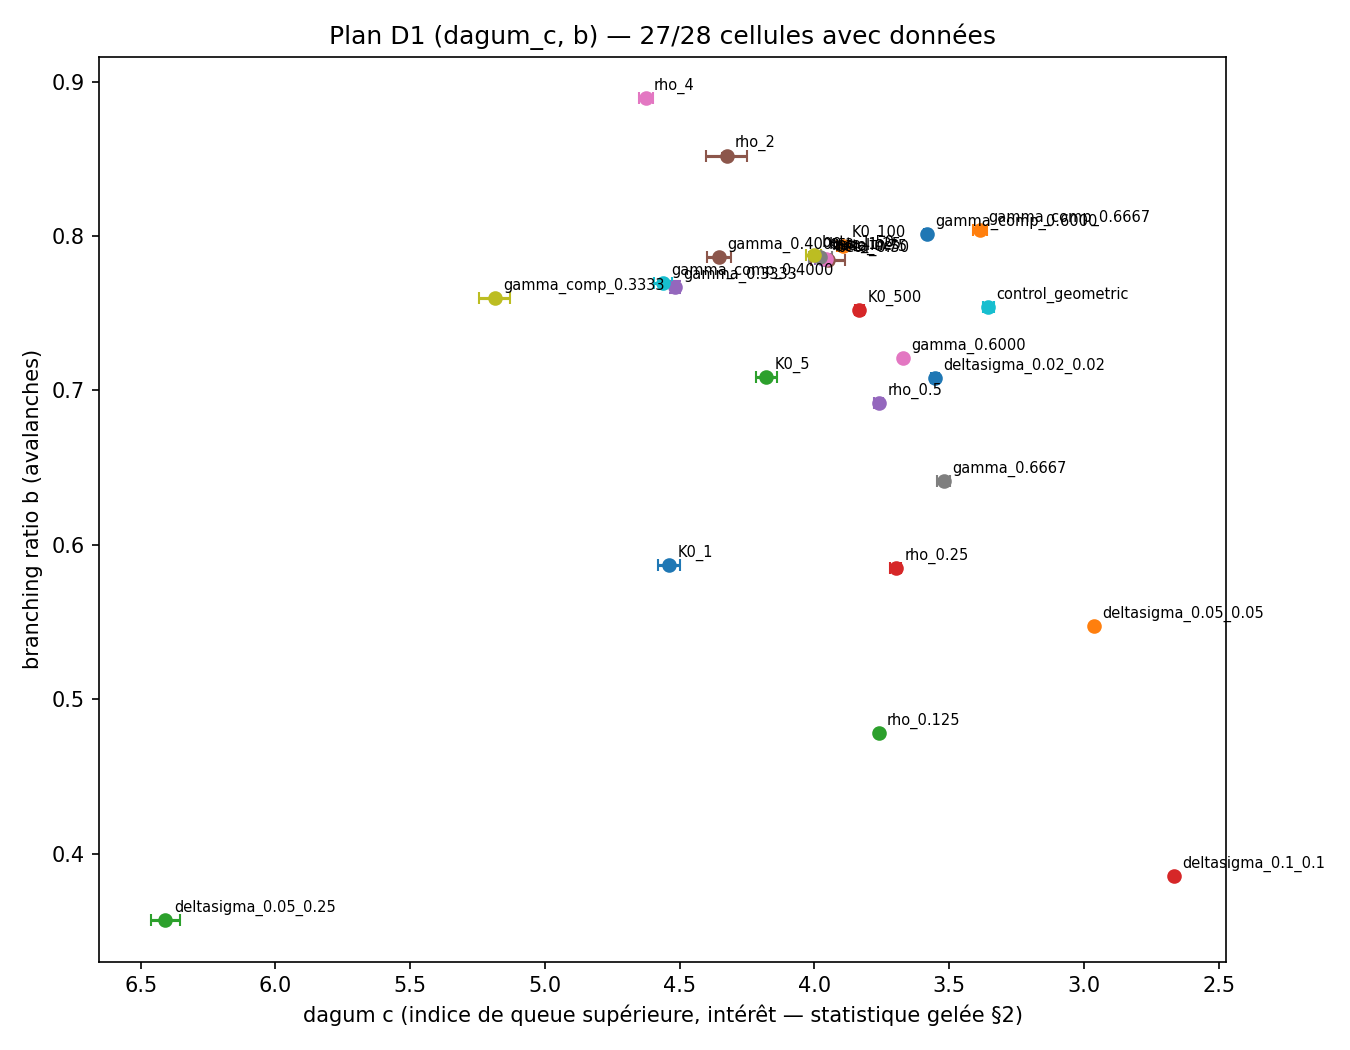
\includegraphics[width=0.95\textwidth]{figures/d1_plan_dagum_c_vs_b.png}
\caption{Plan D1 : un point par cellule, barres d'erreur inter-graines,
axe \code{dagum\_c} inversé pour lire « queue plus épaisse » de gauche à
droite. Table complète : \code{results/d1/d1\_verdict\_cells.csv}.}
\end{figure}

Sur les 26 cellules comparées à la baseline (K0\_2000 exclue, sévère,
\S\ref{sec:k02000}) : 24 confirment l'anti-corrélation ou montrent les
deux métriques bougeant ensemble (non informatif). \textbf{2 cellules ---
\code{gamma\_comp\_0.6000} et \code{gamma\_comp\_0.6667}} ($\gamma=0{,}6$
et $2/3$, $K_0$ compensé pour tenir $K_0/\Kaut(\gamma)$ constant) ---
montrent le motif inverse, avec une tendance MONOTONE sur toute la
branche $\gamma\in\{1/3, 0{,}4, 0{,}6, 2/3\}$ (\code{dagum\_c}:
$5{,}19\to4{,}56\to3{,}58\to3{,}39$ ; $b$:
$0{,}760\to0{,}770\to0{,}802\to0{,}804$), séparation $\sim$15$\sigma$
contre la baseline.

\begin{figure}[H]
\centering
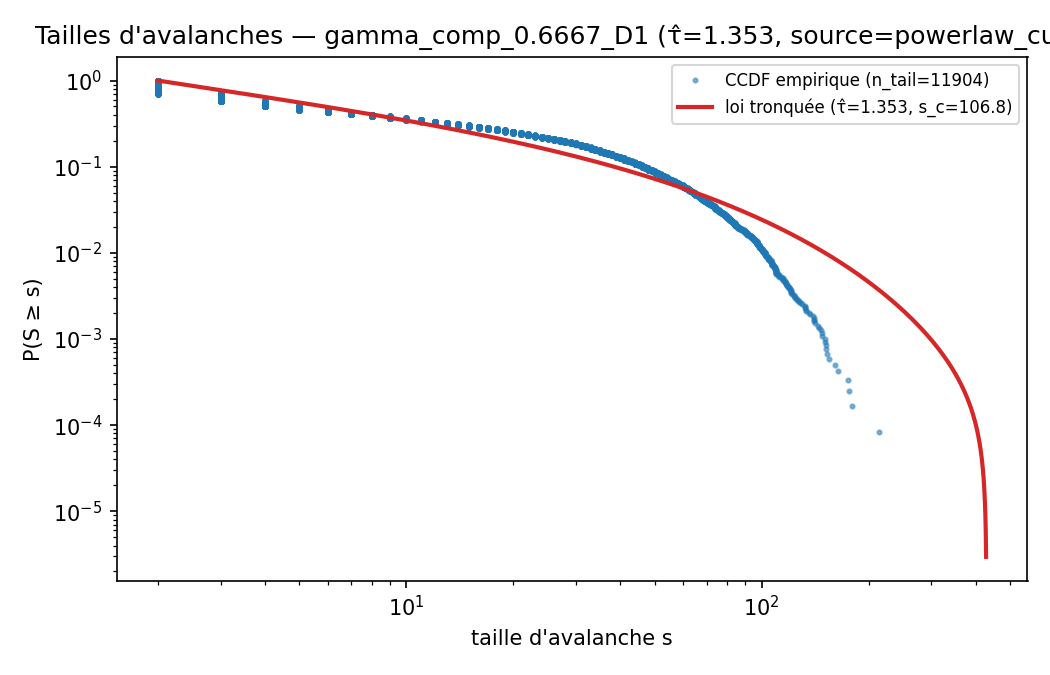
\includegraphics[width=0.8\textwidth]{figures/verification/avalanches_gamma_comp_0.6667_D1.png}
\caption{CCDF des tailles d'avalanches et loi ajustée, \code{gamma\_comp\_0.6667}
(D1, $\lambda=30$).}
\end{figure}

\begin{figure}[H]
\centering
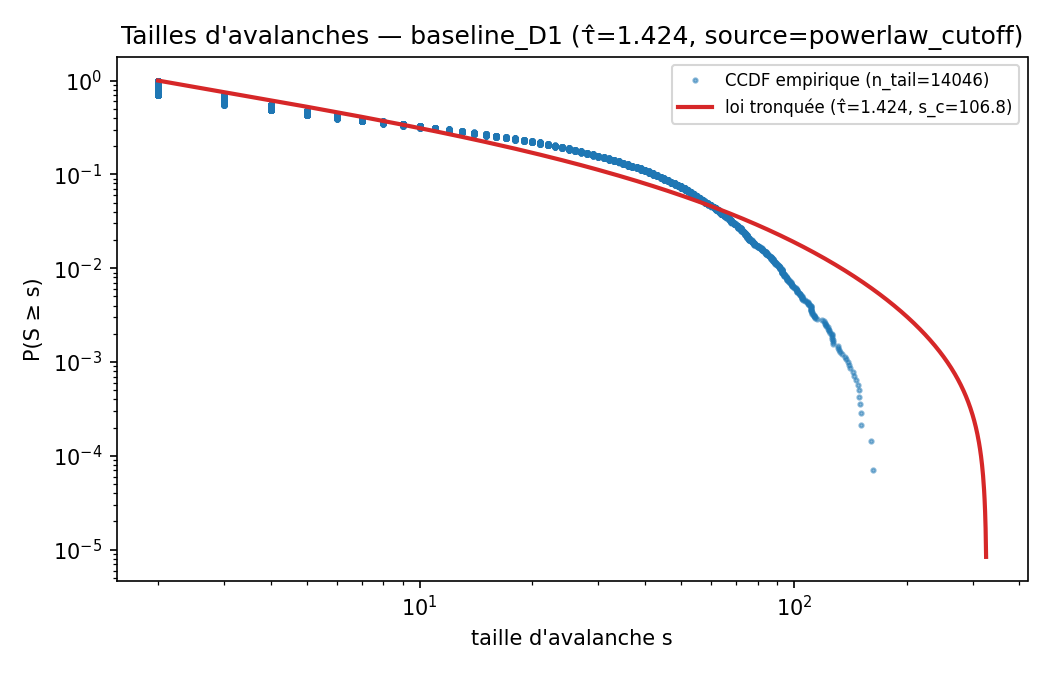
\includegraphics[width=0.8\textwidth]{figures/verification/avalanches_baseline_D1.png}
\caption{CCDF des tailles d'avalanches et loi ajustée, baseline (D1,
$\lambda=30$) --- $\hat\tau=1{,}424$, concorde exactement avec la table
D1 (\code{JOURNAL.md} \S12).}
\end{figure}

\textbf{Réserve appliquée avant de conclure} : \code{gamma\_comp} fait
varier $K_0$ (par construction), donc la population finale varie
d'environ $\pm25\,\%$ autour de la baseline. Ce candidat n'a été traité
comme confirmé qu'après la vérification de taille indépendante
(\S\ref{sec:d3}).

\section{K0\_2000 : échec mémoire propre, résolu, mais cellule intrinsèquement sévère}
\label{sec:k02000}

Détail complet en \S\ref{sec:incidents}. Résumé du résultat scientifique
: \code{dagum\_c} non disponible (3/3 graines sévères), mais le rapport
de branchement reste identifiable (moins sensible à la fenêtre) :
$b = 0{,}6797 \pm 0{,}0011$ (2/3 graines identifiables).

\section{D3 --- robustesse de taille et temporelle du candidat \code{gamma\_comp} : POSITIF}
\label{sec:d3}

\begin{table}[H]
\centering
\begin{tabular}{lccc}
\toprule
$\lambda$ & pop (baseline / gamma\_comp) & $\Delta c$ & $\Delta b$ \\
\midrule
10 & 393 / 468 & $-0{,}5935$ (27,7$\sigma$) & $+0{,}0184$ (8,7$\sigma$) \\
30 & 1163 / 1395 & $-0{,}5819$ (26,4$\sigma$) & $+0{,}0184$ (25,9$\sigma$) \\
100 & 3775 / 4681 & $-0{,}5944$ (84,5$\sigma$) & $+0{,}0185$ (36,9$\sigma$) \\
\bottomrule
\end{tabular}
\end{table}

\textbf{$\Delta b$ est identique à 4 chiffres significatifs sur les trois
échelles} malgré un facteur $>10\times$ sur la population absolue ---
signature attendue d'un effet indépendant de la taille.

\begin{figure}[H]
\centering
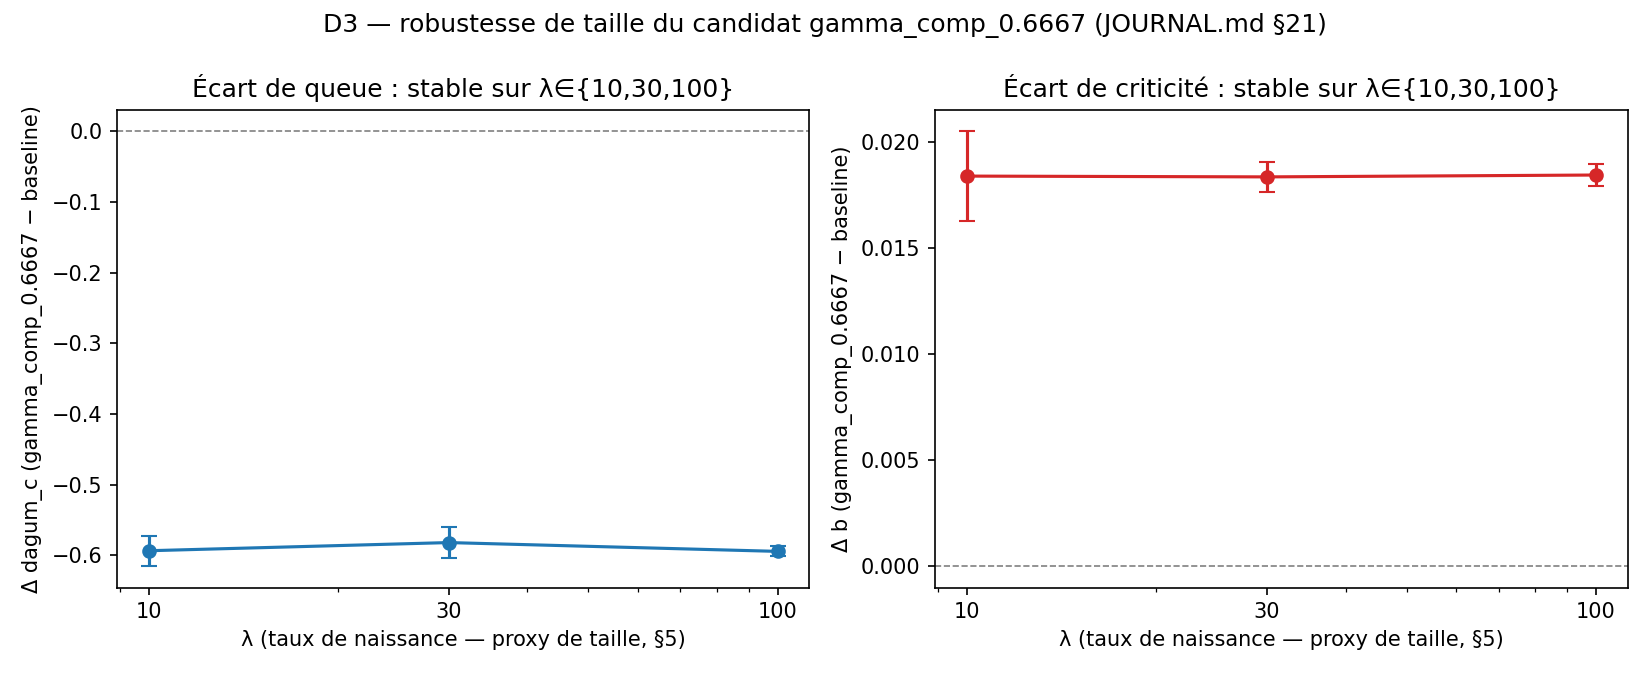
\includegraphics[width=0.95\textwidth]{figures/d3_size_robustness.png}
\caption{$\Delta c$ et $\Delta b$ (\code{gamma\_comp}$-$baseline) contre
$\lambda$, échelle log, barres d'erreur inter-graines. Les deux courbes
sont visuellement plates.}
\end{figure}

Vérification annexe~: la baseline elle-même est size-indépendante sur ces
deux métriques (écart $<1\,\%$ sur $c$, $<0{,}5\,\%$ sur $b$ entre
$\lambda=10$ et $100$) --- reproduit le résultat déjà établi par M4B,
validation indépendante que le test de taille par $\lambda$ fonctionne
comme attendu sur ce moteur.

\textbf{Robustesse temporelle} (distincte de la reproductibilité
inter-graines) : la fenêtre post-convergence découpée en deux moitiés
temporelles donne un écart $b$ stable ($+0{,}0189$ en première moitié,
$+0{,}0178$ en seconde) --- pas un artefact d'une sous-période
particulière.

\subsubsection*{Vérification sur données réelles : \code{gamma\_comp\_0.6667}}

Les figures D1/D3 ci-dessus réutilisaient un pipeline léger (dagum\_c seul,
pas le ladder complet) et supprimaient les instantanés bruts après
analyse (\S\ref{sec:incidents}) --- aucune figure de régression n'était
donc possible pour la cellule centrale sans re-simuler. Un run de
vérification dédié (\code{results/pilot/gamma\_comp\_0.6667\_verif},
$T=8000$, mêmes paramètres que la cellule D1) a été relancé spécifiquement
pour récupérer les instantanés et produire les figures ci-dessous, avec
le même pipeline que \code{baseline\_arithmetic}/\code{control\_geometric}
plus haut.

\begin{figure}[H]
\centering
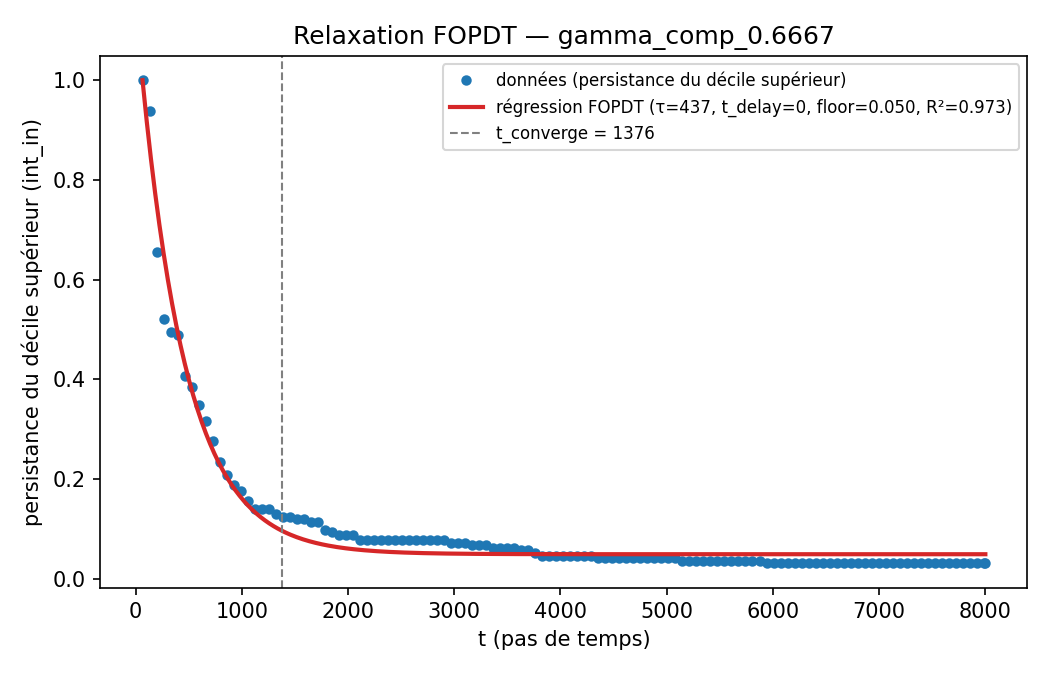
\includegraphics[width=0.8\textwidth]{figures/verification/fopdt_gamma_comp_0.6667.png}
\caption{Relaxation FOPDT, \code{gamma\_comp\_0.6667} (seed 0).
$\tau=436{,}6$, $t_{\mathrm{delay}}\approx0$, $R^2=0{,}973$,
$t_{\mathrm{converge}}=1376$.}
\end{figure}

\begin{figure}[H]
\centering
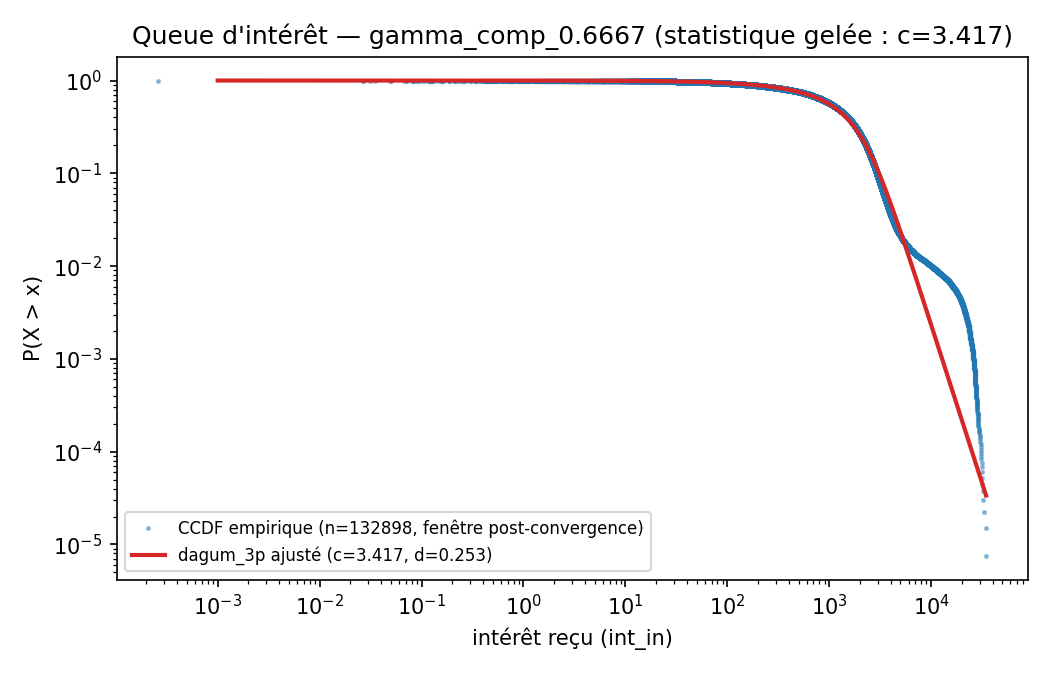
\includegraphics[width=0.8\textwidth]{figures/verification/dagum_tail_gamma_comp_0.6667.png}
\caption{CCDF empirique de \code{int\_in} (fenêtre post-convergence) et
survie \code{dagum\_3p} ajustée, \code{gamma\_comp\_0.6667} (seed 0) :
$c=3{,}417$ --- cohérent avec la queue nettement plus fine que la
baseline mesurée sur les 3 graines D1 (\S\ref{sec:d3}, $\Delta c\approx-0{,}58$
à $\lambda=30$, ce run isolé confirmant l'ordre de grandeur sur données
brutes indépendantes du pipeline léger).}
\end{figure}

\textbf{Verdict D3 : POSITIF.} \code{gamma\_comp\_0.6667} casse
l'anti-corrélation de façon robuste à la taille ET à la fenêtre
temporelle. C'est le premier résultat de tout le programme M4.2B$\to$M4.3
(65 cellules testées) qui casse l'anti-corrélation avec cette solidité
statistique. Mécanisme : $\gamma$ et la compensation $K_0/\Kaut(\gamma)$
sont déjà dans le moteur --- aucune ablation de mécanisme n'est
nécessaire pour ce résultat spécifique.

\section{Décision d'ablation : jalon atteint, décision réservée à la supervision}
\label{sec:ablation}

La cartographie D1 est le jalon fixé à l'avance pour trancher, par écrit,
si une refonte de mécanisme (famille de moyennes de puissance pour la
règle de taux) est nécessaire. \textbf{Cette décision est explicitement
hors du périmètre de ce qui peut être tranché de façon autonome}, même
après confirmation D3.

\textbf{La question concrète, pour vous} : trois options, de la moins à
la plus coûteuse :
\begin{itemize}
\item[(a)] \textbf{S'arrêter ici.} Le résultat répond déjà à la question
  du prompt.
\item[(b)] \textbf{Affiner le balayage $\gamma_{\mathrm{comp}}$ déjà
  implémenté} ($\gamma\in\{0{,}7\,;0{,}8\,;0{,}9\}$ compensé) --- pas une
  ablation, coût $\approx$identique à une cellule D1 (quelques heures).
\item[(c)] \textbf{Engager le code de mécanisme nouveau} anticipé par le
  prompt (famille de moyennes de puissance pour la règle de taux) ---
  investissement de code réel, ablation propre requise.
\end{itemize}

Mon inclination technique, pour ce qu'elle vaut : \textbf{(b) avant (c)},
parce que (b) est presque gratuit avec l'outillage déjà en place et
répond à une partie de la question que (c) chercherait aussi à répondre.

\section{Complément : accessibilité \code{simulation\_lab}, bins adaptatifs, run de démonstration}
\label{sec:complement}

Trois demandes utilisateur successives, distinctes du calcul D1/D2/D3
(déjà clos \S\ref{sec:d3}-\ref{sec:ablation}) : (a) toutes les
simulations ont-elles leurs graphiques \code{simulation\_lab}, triés par
cellule ? (b) tous les histogrammes doivent avoir des bins de taille
adaptative ; (c) un run de démonstration avec toutes les figures y
compris les vies individuelles.

\textbf{(a)} Réponse initiale : non --- \S8 du prompt demandait de
réutiliser \code{simulation\_lab} tel quel, ce qui n'avait pas été fait
(aucun adaptateur M4.3), et le nettoyage disque post-analyse de D1/D3
supprimait les instantanés bruts \emph{avant} toute génération de figures
possible. Mesures réelles avant correctif : \code{individual\_series}
n'est utilisé que par 1 des 9 recettes de figures et
\code{individual\_every=0} est la convention de toute la campagne M4.2B
elle-même ; \code{loan\_events.csv.gz} (${\sim}65\,\%$ du poids d'un run)
n'est utilisé par aucune des 28 figures. Seul \code{snapshots/} manquait
réellement. Correctif : adaptateur créé
(\code{modeles-systeme-physicoeconomique/m4\_3\_credit\_soc/}), les 96
runs D1+D3 relancés avec figures générées \emph{avant} le nettoyage
disque --- en cours à la date de rédaction (\code{JOURNAL.md} \S24).

\textbf{(b)} Deux occurrences du même défaut trouvées et corrigées dans
\code{reporting.py} (copie M4.3 uniquement, pas répercuté sur l'original
M4.2B) : \code{temporal\_density()} (figures \code{*\_evolution.gif} et
\code{*\_temporal\_mean.png}) et un histogramme local dans
\code{network\_figure()} avaient un nombre de bins adaptatif mais des
bornes espacées uniformément en log --- sur des champs à queue lourde, ça
produit un bruit de comptage qui domine le signal. Remplacé par les
mêmes bornes aux quantiles empiriques que \code{adaptive\_hist()}
(déjà correcte).

\begin{figure}[H]
\centering
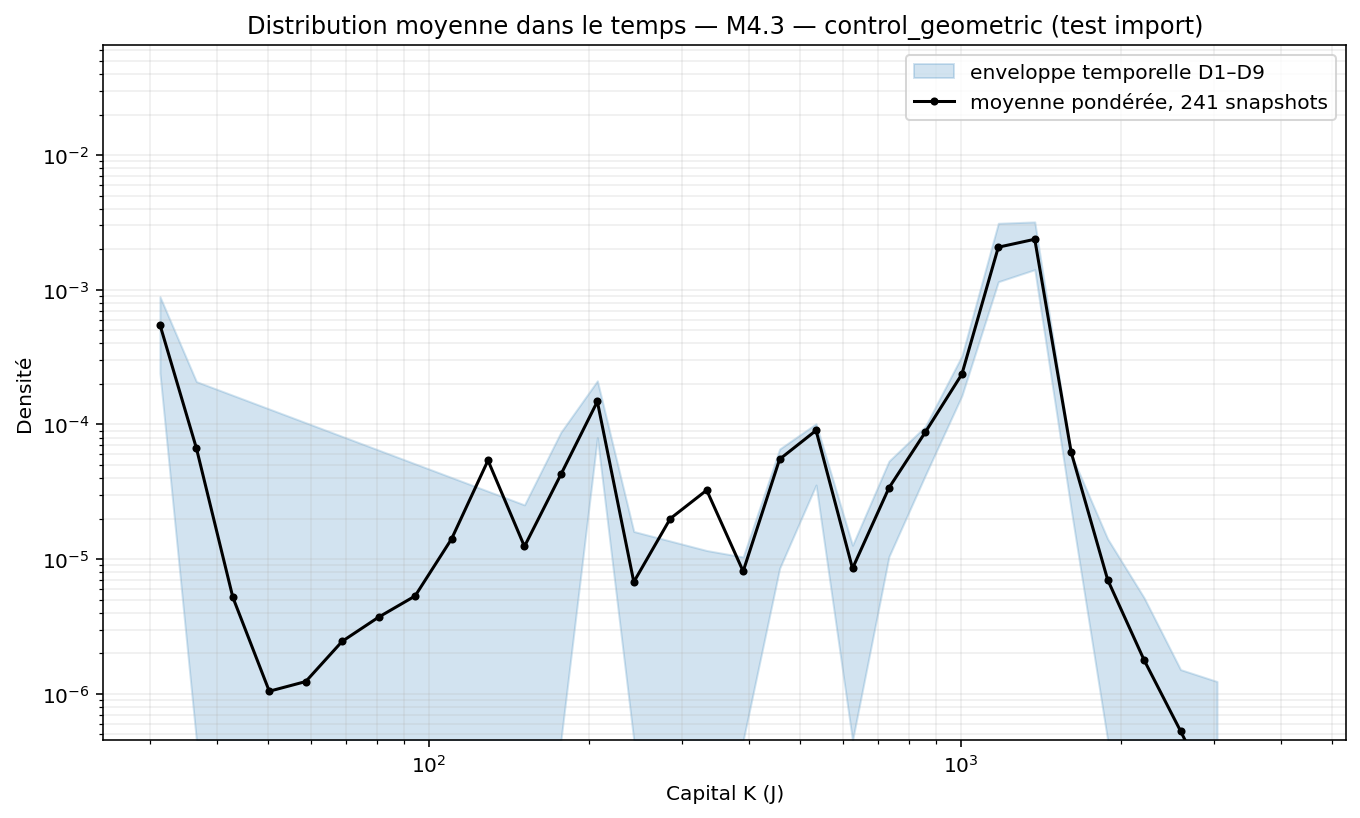
\includegraphics[width=0.48\textwidth]{figures/verification/bins_fix_before.png}
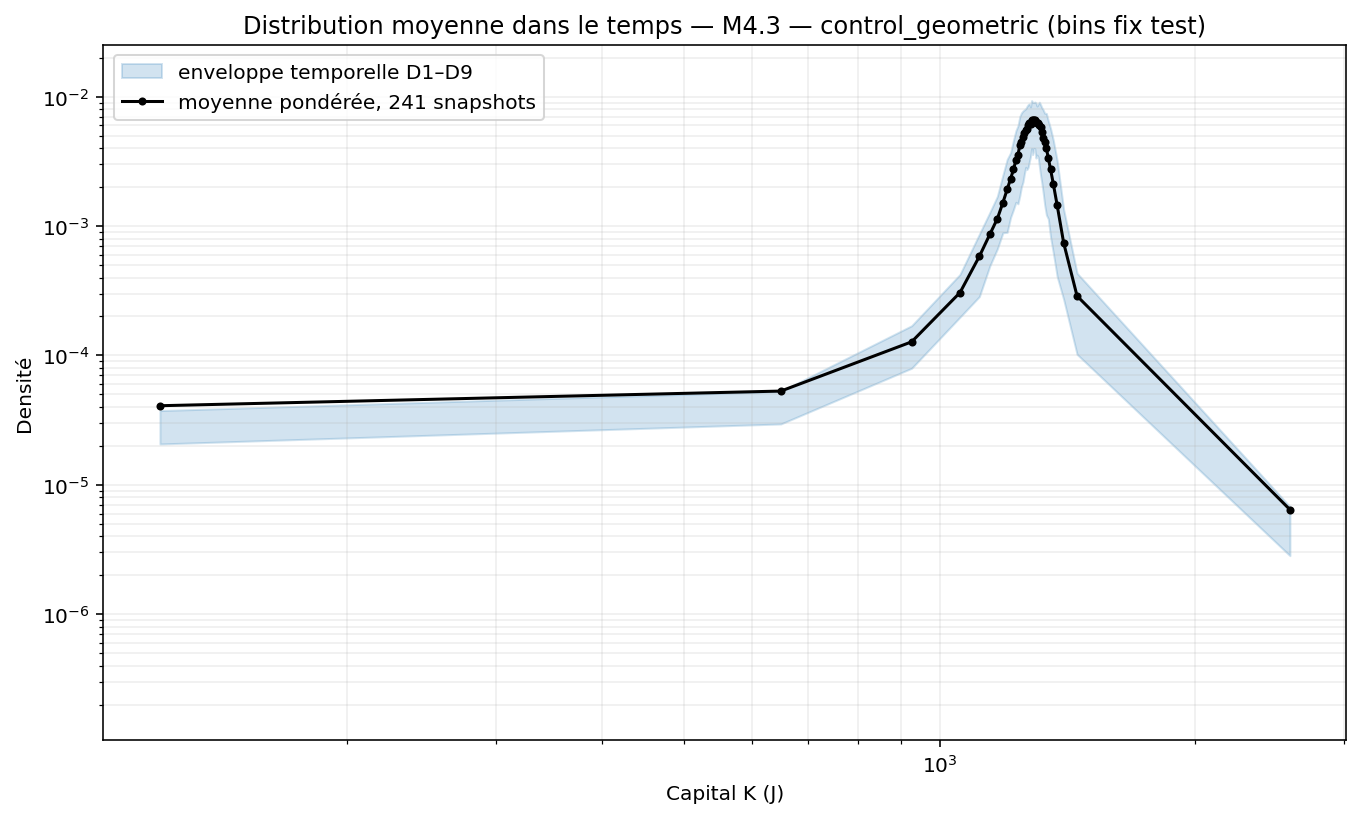
\includegraphics[width=0.48\textwidth]{figures/verification/bins_fix_after.png}
\caption{\code{entity\_size\_histo\_temporal\_mean.png},
\code{control\_geometric}/seed 0, avant (gauche, bornes log uniformes) et
après (droite, bornes aux quantiles) le correctif. Mêmes données, même
fonction appelante --- seul le choix des bornes change.}
\end{figure}

\textbf{(c)} \code{results/pilot/baseline\_showcase} (cellule baseline,
$T=8000$, \code{individual\_every=1} --- première fois dans ce programme) :
32 figures générées sans erreur y compris les vies individuelles,
impossibles sans \code{individual\_series} peuplé. Données brutes
nettoyées ensuite (1,6 Go $\to$ 53 Mo).

\begin{figure}[H]
\centering
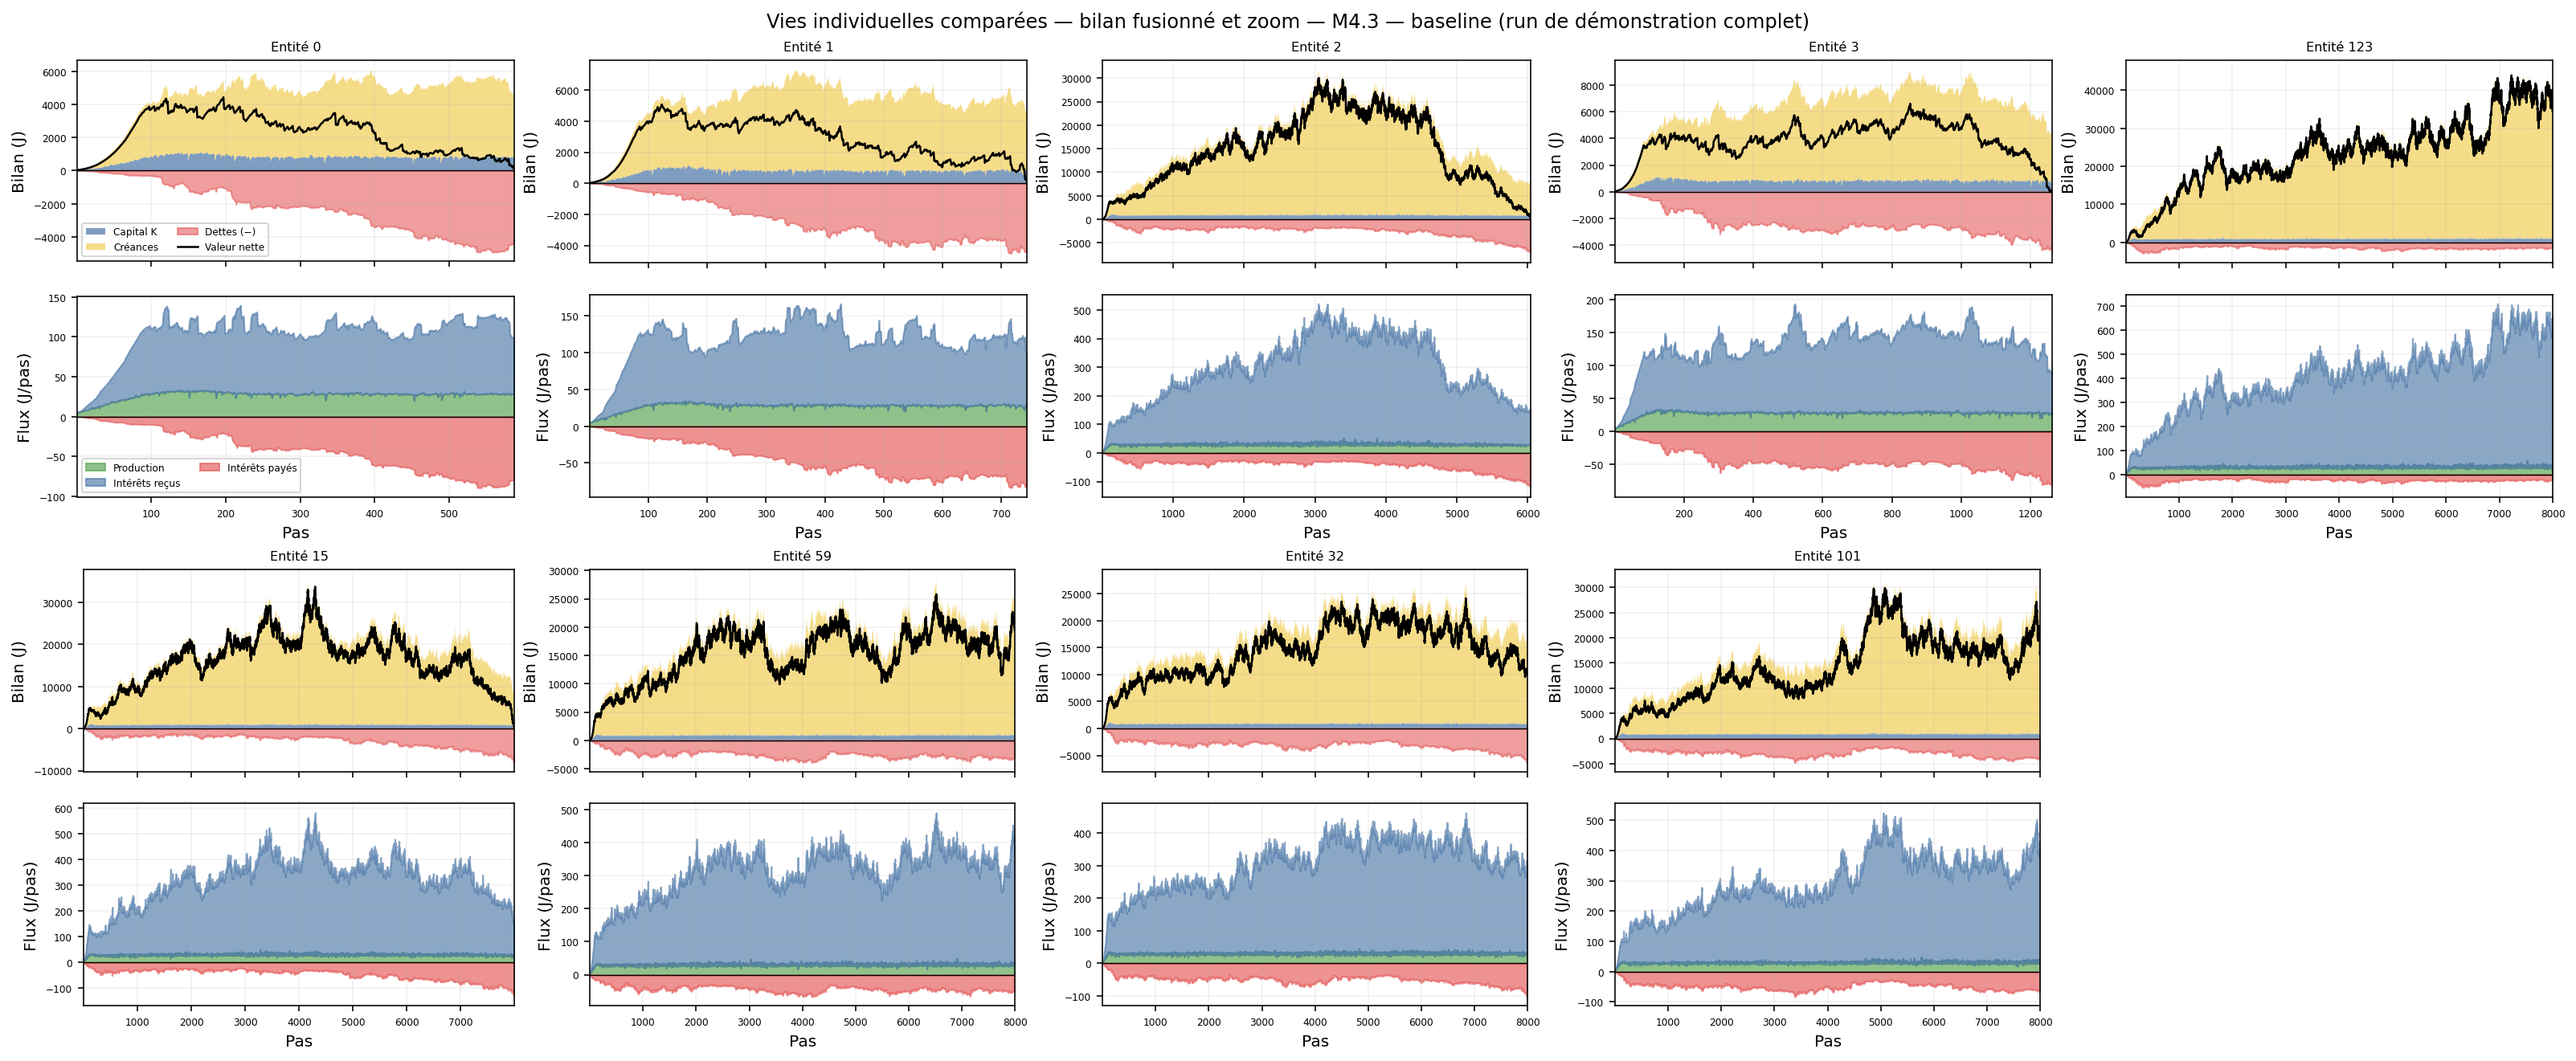
\includegraphics[width=0.95\textwidth]{figures/showcase_entity_lives.png}
\caption{Vies individuelles comparées, run de démonstration baseline
(seed 0) --- bilan (haut) et flux (bas) pour 9 entités sélectionnées
(naissance précoce, taille maximale, longévité).}
\end{figure}

Ces trois points sont des correctifs d'outillage/de processus, pas de
nouveaux résultats scientifiques --- ils ne changent rien au verdict
D2/D3 ni à la décision d'ablation, toujours en attente de votre
arbitrage.

\section{Limites et non testé à ce stade}

\begin{itemize}
\item Statistique de queue gelée sur 3 graines par régime --- assez pour
  trancher entre les deux candidats testés, pas assez pour une
  incertitude publiable au sens strict (M4.2B utilisait 5 graines de
  confirmation disjointes).
\item La robustesse temporelle n'a été vérifiée que sur la paire
  baseline/gamma\_comp\_0.6667 à $\lambda=30$, pas sur les 28 cellules de
  D1.
\item La coupure d'avalanche $\hat s_c(\lambda)$ n'a pas encore été
  ré-établie sur ce moteur.
\item $b$ et $\hat\tau$ utilisent $s_{\min}=2$ (convention M4B/M4.2B)
  sans re-test de sensibilité à ce choix dans M4.3.
\item Le mécanisme de reprise depuis checkpoint (testé et fonctionnel)
  n'a jamais eu besoin d'être exercé en pratique.
\end{itemize}

\bigskip
\noindent\emph{Document généré et maintenu par le programme autonome
M4.3. Détail chronologique complet, horodaté, dans \code{JOURNAL.md}.
Code source (\code{scripts/}, \code{m4\_3/}) disponible dans le dépôt
local, pas encore versionné dans Git (même convention que M4.2B) ---
demander si nécessaire.}

\end{document}
